\documentclass[modern,twocolumn]{aastex631}

\usepackage{xspace}

\usepackage{xcolor, fontawesome}
\definecolor{twitterblue}{RGB}{64,153,255}

\newcommand{\twitter}[1]{\href{https://twitter.com/#1 }{\textcolor{twitterblue}{\faTwitter}\,\tt \textcolor{twitterblue}{@#1}}}

\newcommand{\github}[1]{\href{https://github.com/#1 }{\textcolor{black}{\faGithub}\,\tt \textcolor{black}{#1}}}

\newcommand{\tess}{\textit{TESS}}
\newcommand{\sname}{V1298~Tau\xspace}
\newcommand{\allplanets}{V1298~Tau~bcde\xspace}
\newcommand{\planetb}{V1298~Tau~b\xspace}
\newcommand{\planetc}{V1298~Tau~c\xspace}
\newcommand{\planetd}{V1298~Tau~d\xspace}
\newcommand{\planete}{V1298~Tau~e\xspace}
\newcommand{\planetknown}{V1298~Tau~bcd\xspace}
\newcommand{\rearth}{$R_\oplus$\xspace}
\newcommand{\exoplanet}{\texttt{exoplanet}\xspace}



\submitjournal{AJ}


\shorttitle{V1298 Tau with \tess}
\shortauthors{Feinstein et al.}


\begin{document}

\title{V1298~Tau with TESS: Updated Ephemerides, Radii, and Period Constraints from a Second Transit of V1298~Tau~e}

\author[0000-0002-9464-8101]{Adina~D.~Feinstein}
\altaffiliation{NSF Graduate Research Fellow}
\affiliation{Department of Astronomy and Astrophysics, University of Chicago, Chicago, IL 60637, USA}

\author[0000-0001-6534-6246]{Trevor J.\ David}
\affiliation{Center for Computational Astrophysics, Flatiron Institute, New York, NY 10010, USA}
\affiliation{Department of Astrophysics, American Museum of Natural History, New York, NY 10024, USA}

\author[0000-0001-7516-8308]{Benjamin~T.~Montet}
\affiliation{School of Physics, University of New South Wales, Sydney, NSW 2052, Australia}
\affiliation{UNSW Data Science Hub, University of New South Wales, Sydney, NSW 2052, Australia}

\author[0000-0002-9328-5652]{Daniel Foreman-Mackey}
\affiliation{Center for Computational Astrophysics, Flatiron Institute, New York, NY 10010, USA}

\author[0000-0002-4881-3620]{John~H.~Livingston}
\affiliation{Department of Astronomy, University of Tokyo, 7-3-1 Hongo, Bunkyo-ku, Tokyo 113-0033, Japan}

\author[0000-0003-3654-1602]{Andrew~W.~Mann}
\affiliation{1Department of Physics and Astronomy, The University of North Carolina at Chapel Hill, Chapel Hill, NC 27599, USA}


\correspondingauthor{Adina~D.~Feinstein;\\ \twitter{afeinstein20}; \github{afeinstein20};} \email{afeinstein@uchicago.edu} 

%%%%%%%%%%%%%%%%%%%%
% abstract must be < 250 words
% currently at 180 words
%%%%%%%%%%%%%%%%%%%%
\begin{abstract}

\sname is a young (20--30~Myr) solar analogue hosting four transiting exoplanets with sizes between $0.5 - 0.9 R_J$. Given the system's youth,  it provides a unique opportunity to understand the evolution of planetary radii at different separations in the same stellar environment. \sname was originally observed 6 years ago during \textit{K2} Campaign 4. Now, \sname has been re-observed during the extended mission of NASA's Transiting Exoplanet Survey Satellite (\tess). Here, we present new photometric observations of \sname from the 10-minute \tess\ Full-Frame Images. We use the \tess\ data to update the ephemerides for \allplanets as well as compare newly observed radii to those derived from the \textit{K2} light curve, finding shallower transits for \planetknown in the redder \tess\ bandpass at the $1-2\sigma$ level. We suspect the difference in radii is due to starspot-crossing events or contamination from nearby faint stars on the same pixels as \sname. We additionally catch a second transit of \planete and present a new method for deriving the marginalized posterior probability of a planet's period from two transits observed years apart. We find the highest probability period for \planete to be in a near 2:1 mean motion resonance with \planetb which, if confirmed, could make \allplanets a 4 planet resonant chain. \sname is the target of several ongoing and future observations. These updated ephemerides will be crucial for accurately recovering transit events and understanding any future Doppler tomographic or transmission spectroscopy signals.

\end{abstract}

%%%%%%%%%%%%%%%%%%%%

\keywords{Exoplanets (498) --- Pre-main sequence (1289) --- Starspots (1572) --- Stellar activity (1580)}

%%%%%%%%%%%%%%%%%%%%

\section{Introduction} \label{sec:intro}
Planetary radii are expected to evolve over time, due to a variety of endogenous and exogenous physical processes, such as gravitational contraction, atmospheric heating and mass-loss, and core-envelope interactions \citep[e.g.][]{OwenWu2013, Lopez2013, Jin2014, ChenRogers2016, Ginzburg2018}. The most dramatic changes are believed to occur at early stages, when planets are still contracting and radiating away the energy from their formation, and when host stars are heating planetary atmospheres with high levels of X-ray and ultraviolet radiation. Since the size evolution of any individual planet is believed to be slow relative to typical observational baselines, the best way to make inferences about the size evolution of exoplanets is by measuring the sizes of large numbers of planets across a range of ages. 

NASA's Transiting Exoplanet Survey Satellite \citep[\tess;][]{Ricker2015} has made significant inroads toward this objective. \tess's observations of $\sim 90 \%$ of the sky have allowed for exoplanet transit searches around stars ranging from the pre-main sequence to the giant branch. It is through targeted surveys of young stars such as the THYME \citep[e.g.][]{Newton2019}, PATHOS \citep[e.g.][]{Nardiello2020}, and CDIPS \citep[e.g.][]{Bouma2020} surveys, along with case studies of individual systems \citep[e.g.][]{benatti19, Plavchan2020, Hedges2021, Zhou2021} that the timeline for planetary radii evolution can be pieced together. 

The \sname planetary system is one particularly valuable benchmark for understanding the size evolution of exoplanets. \sname is a pre-main sequence, approximately solar-mass star that was observed in 2015 by NASA's \textit{K2} mission \citep{Howell2014}. Analysis of the \textit{K2} data revealed the presence of four transiting planets, all with sizes between that of Neptune and Jupiter \citep{David2019a, David2019b}. There are no other known examples of exoplanetary systems with so many planets larger than Neptune interior to 0.5~au, despite the high completeness of the \textit{Kepler} survey to large ($>5$~\rearth), close-in planets. This observation raises the possibility of a causal connection between the extreme youth of \sname and the uncommonly large sizes of its planets.  

The youth of \sname was initially established on the basis of its strong X-ray emission \citep{Wichmann1996}, high photospheric lithium abundance \citep{Wichmann2000}, and proper motion measurements \citep{frink1997}. An additional recent blind search for co-moving stars using Gaia DR1 astrometry data found \sname was co-moving with 8 other stars \citep[Group 29 in][]{Oh2017}. A kinematic study of the Taurus star-forming region \citet{Luhman2018} used Gaia DR2 data to extended the membership of this group and derived an age of $\sim$~40~Myr. However, more recent analyses based on Gaia EDR3 astrometry suggests \sname may belong to either the D2 or D3 subgroups of Taurus, both of which have estimated ages $\lesssim$10~Myr \citep{gaidos21, Krolikowski2021}. Other studies focused specifically on the \sname system have estimated its age to be 23$\pm$4~Myr from comparison with empirical and theoretical isochrones \citep{David2019b}, or 28$\pm$4~Myr from isochrone fitting to the \citet{Luhman2018} Group 29 membership list given Gaia EDR3 data \citep{johnson21}. While the precise age of \sname remains uncertain, most estimates fall in the 10--40~Myr range and we adopt $t \approx$~20--30~Myr.

Given the system's youth and potential to reveal information about the initial conditions of close-in planetary systems \citep[e.g.][]{Owen2020,Poppenhaeger2021}, \sname has been the target for extensive follow-up observations. These include efforts to constrain planet masses with radial velocities \citep{Beichman2019}, measure the spin-orbit alignments of planet c \citep{Feinstein21} and planet b \citep{johnson21, gaidos21}, measure or constrain atmospheric mass-loss rates for the innermost planets \citep{Schlawin21, Vissapragada21}, and an approved program to study the planetary atmospheres using the James Webb Space Telescope \citep[JWST;][]{Desert2021}.

Here we report on newly acquired \tess\ observations of \sname which help to refine the orbital ephemerides of the transiting planets and enable comparison of the planet sizes inferred from two different telescopes with different bandpasses (\tess\ and \textit{Kepler}). The letter is laid out as follows. We describe the observations and light curve extraction in Section~\ref{sec:observations}. In Section~\ref{sec:analysis}, we present our light curve modeling and method for computing the marginalized posterior probability of a transiting planet's period from two transits observed with a large time gap. In Section~\ref{sec:radii}, we discuss the differences in measured transit parameters between \textit{K2} and \tess\ data and speculate on the causes for different measured radii. We conclude in Section~\ref{sec:conclusions}.

%%%%%%%%%%%%%%%%%%%%%%%%%%%%%%%%%%%%%%%%%%%%%%%%%%%%%%%
\begin{figure}[t!]
\begin{center}
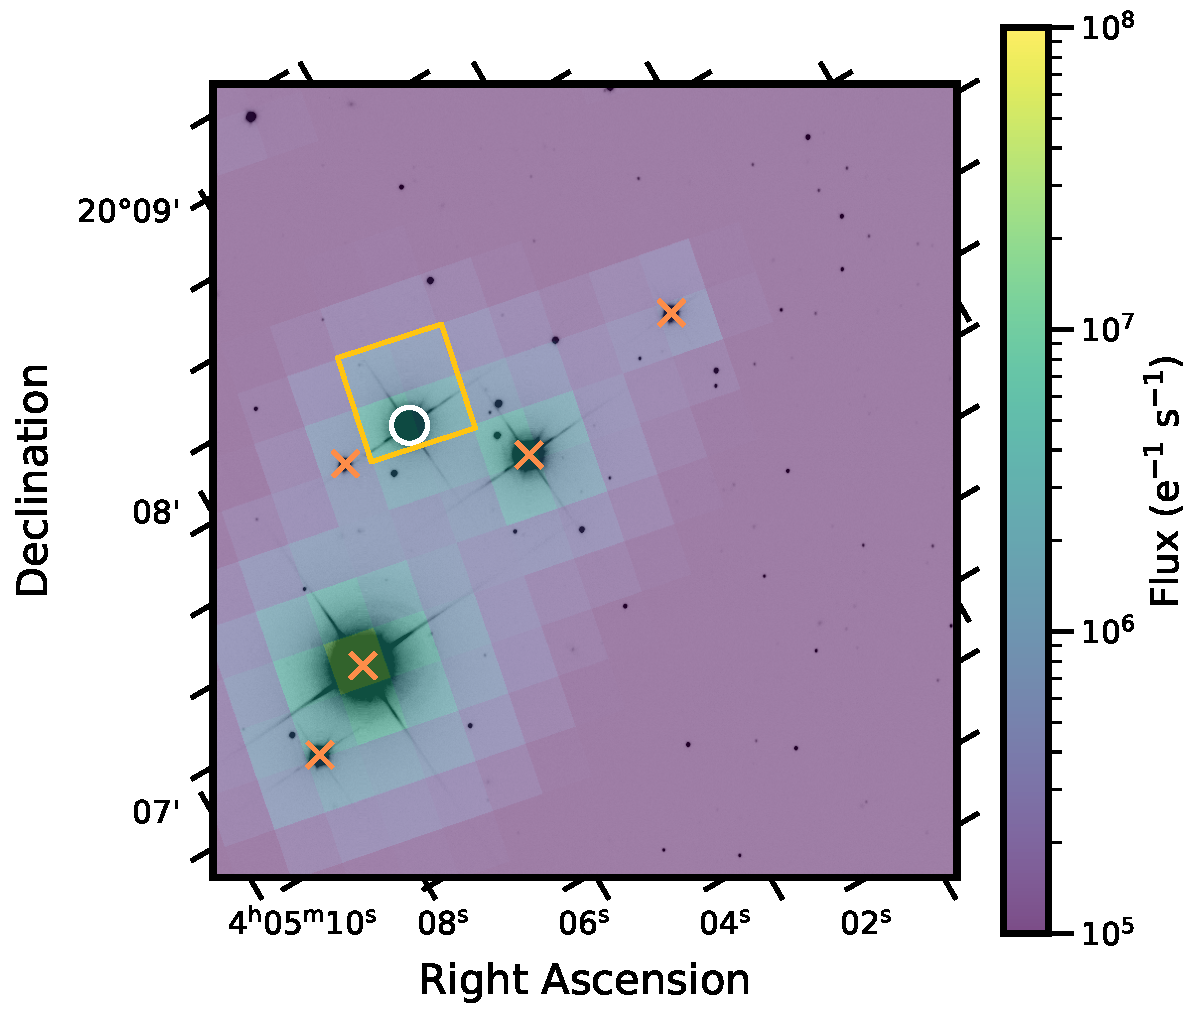
\includegraphics[width=0.46\textwidth,trim={0.25cm 0 0 0}]{static/TESSaperture.pdf}
\caption{The \tess\ \texttt{tica} FFI target pixel file (TPF) overlaid with a sky image of \sname taken with the Digitized Sky Survey (DSS) r-band. \sname is highlighted by the white circle; nearby sources with \tess\ magnitudes $< 14$ are marked with orange x's. There are two bight nearby sources to \sname. While aperture photometry would be feasible for this system (yellow square), we found fitting three point-spread functions to the brightest stars extracted the cleanest light curve for \sname. \href{https://github.com/afeinstein20/v1298tau_tess/blob/main/src/figures/tpf.py}{\github}} \label{fig:tpf}
\end{center}
\end{figure}
%%%%%%%%%%%%%%%%%%%%%%%%%%%%%%%%%%%%%%%%%%%%%%%%%%%%%%%

\section{TESS Observations} \label{sec:observations}

During its Extended Mission Cycle 4, \tess\ is re-observing many of the previous \textit{K2} fields. \sname (TIC 15756231) was observed by \tess\ in Sectors 43 (UT 16 Sep 2021 to UT 12 Oct 2021) at 10-minute cadence within the Full-Frame Images (FFIs). We used the \texttt{tica} \citep{fausnaugh20} software to download calibrated FFIs for Sector 43 and the first orbit of Sector 44, as these FFIs are quickly available after the data is downlinked. 

We created light curves from the \texttt{tica}-processed FFIs by modeling the point-spread function (PSF) of \sname and the two nearby bright sources (see Figure~\ref{fig:tpf}), following the PSF modeling routine in \cite{feinstein19}. In summary, we calculated and maximized the likelihood value of seven parameters per each Gaussian: the $x$ and $y$ width, 2D position, amplitude, a rotational term, and a background term. The Gaussian fits are allowed to vary at each time step. Aperture photometry (example square aperture shown in Figure~\ref{fig:tpf}) provided a light curve with more systematics and scatter. We found that modeling the three brightest stars simultaneously, including \sname, with a 2D Gaussian created the least contaminated light curve. Our extracted light curve is shown in the top row of Figure~\ref{fig:transits}.

%%%%%%%%%%%%%%%%%%%%%%%%%%%%%%%%%%%%%%%%%%%%%%%%%%%%%%%
\begin{figure*}[hbtp]
\begin{center}
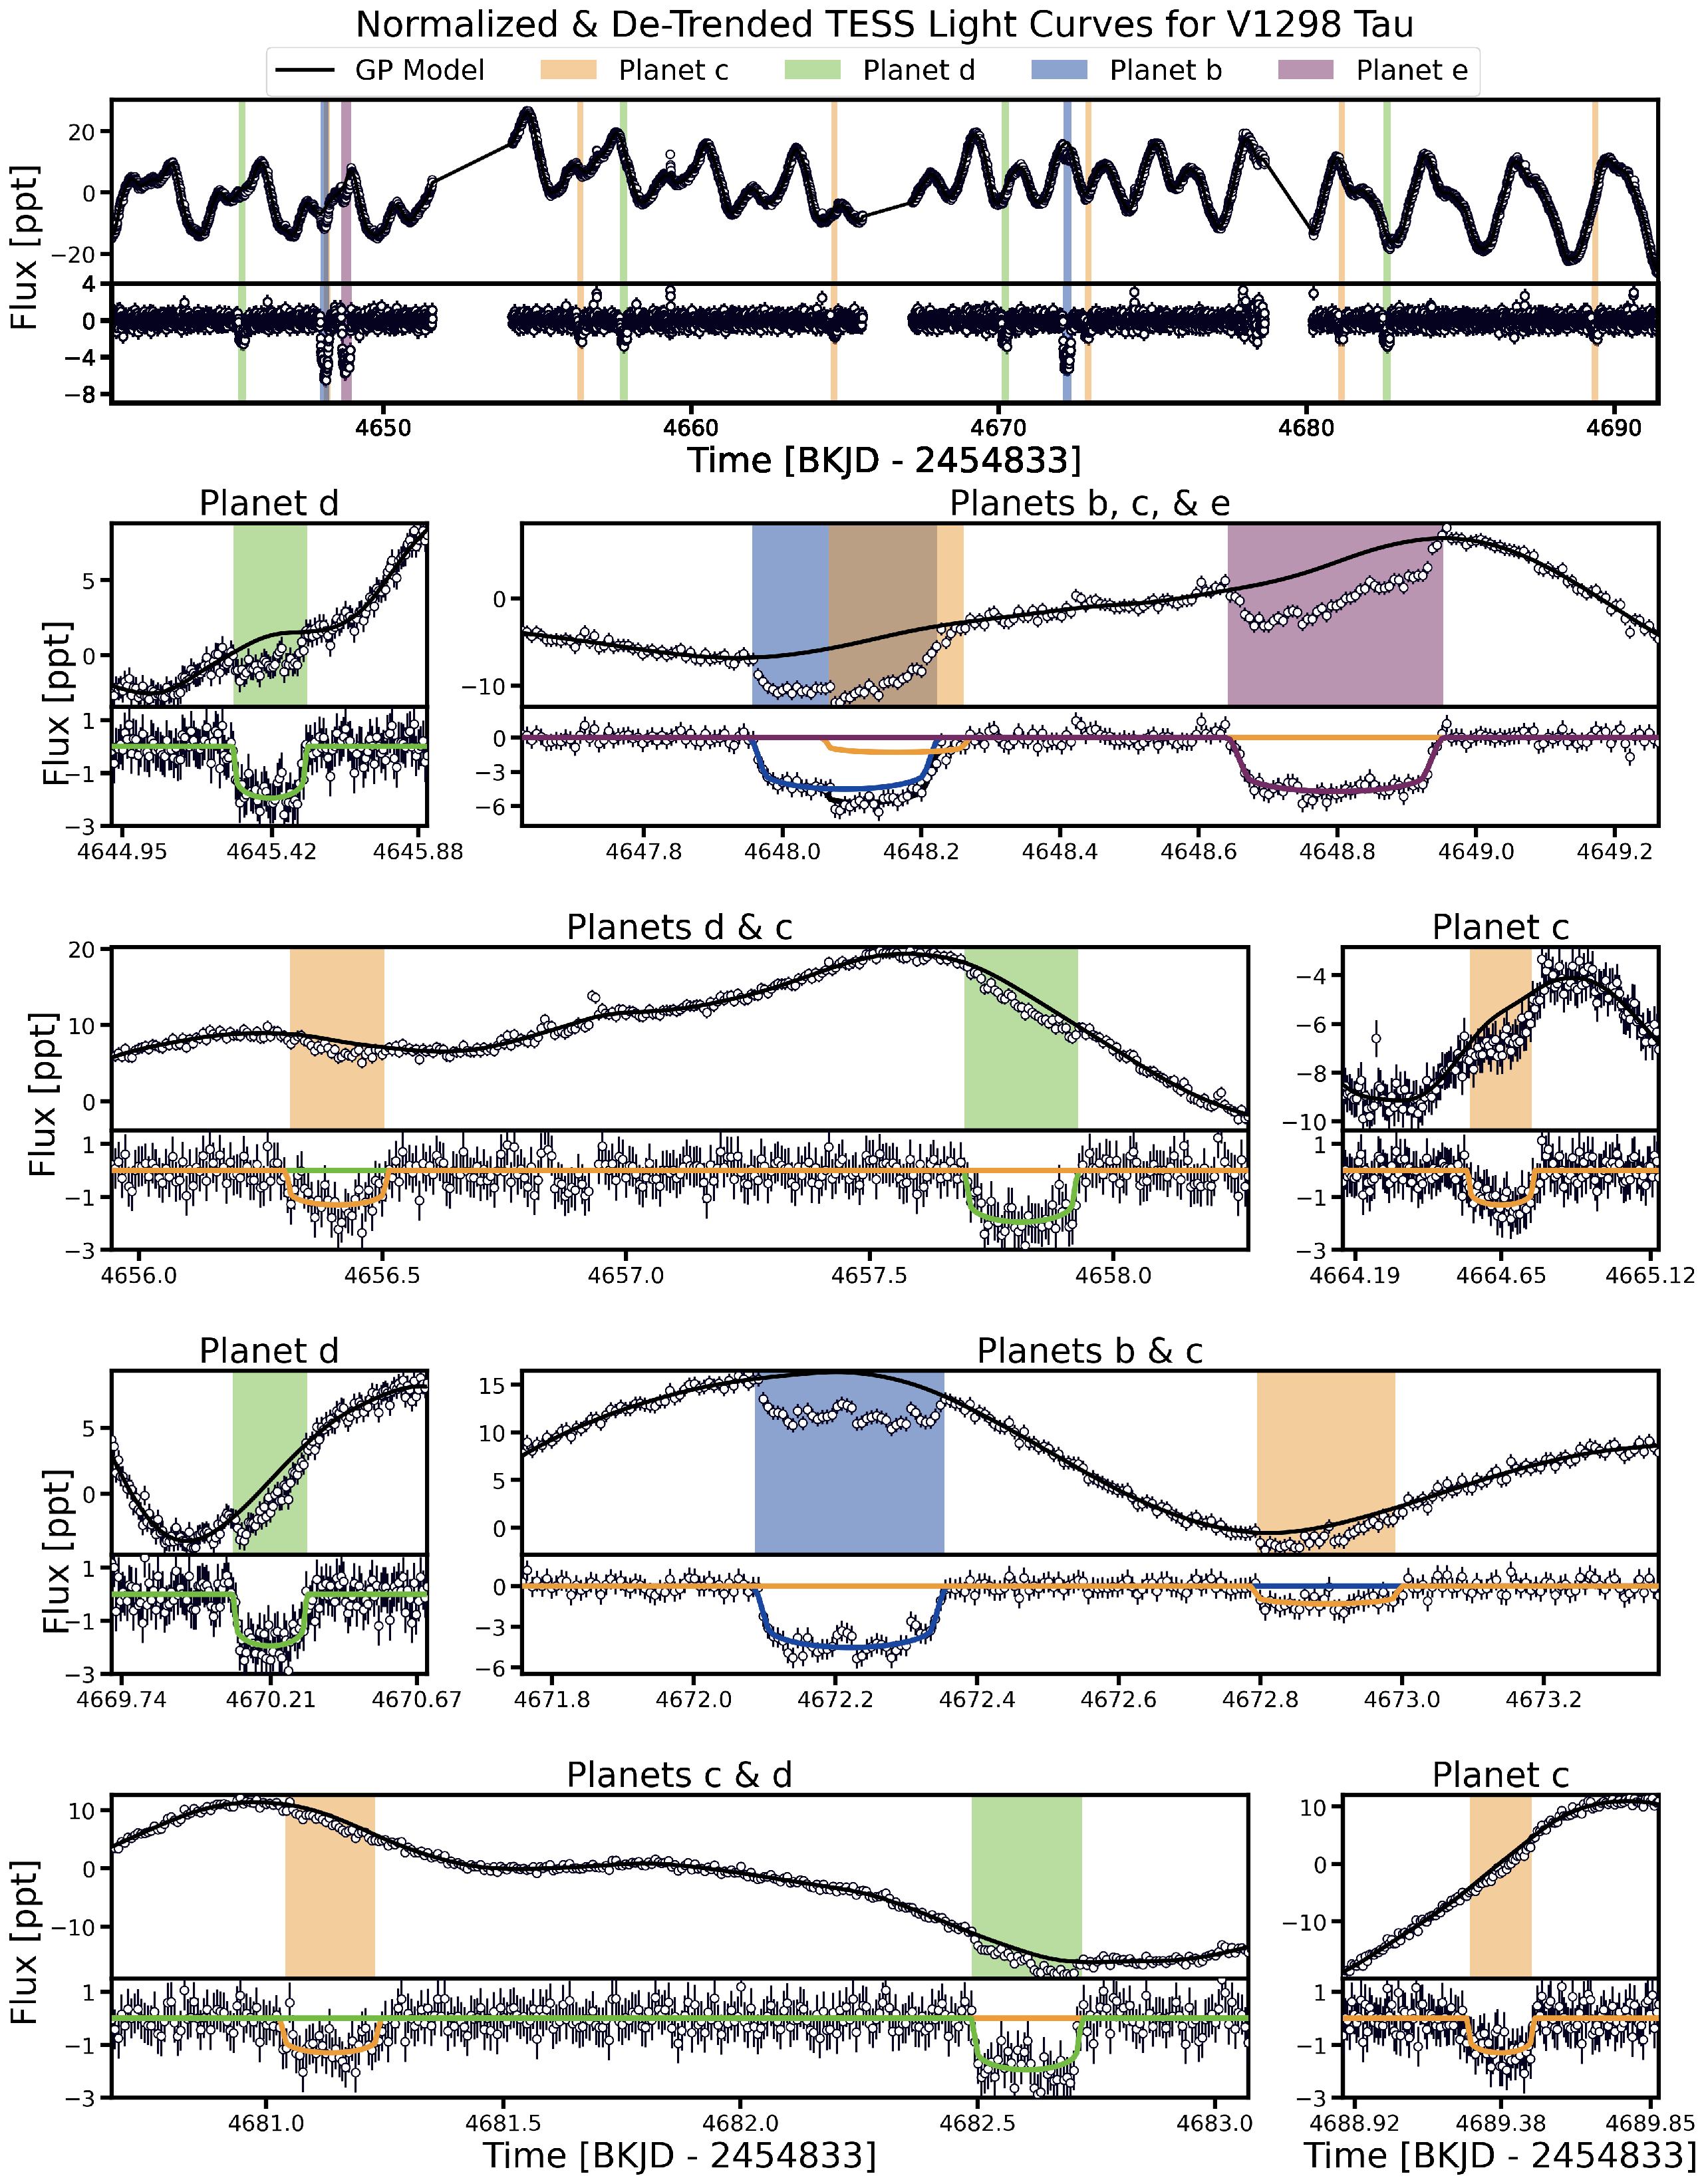
\includegraphics[width=\textwidth,trim={0.25cm 0 0 0}]{figures/transits.pdf}
\caption{\sname extracted light curve from the \texttt{tica}-processed full-frame images for all of Sector 43 and the first orbit of Sector 44, with transits of \allplanets highlighted by color. Each subplot contains the raw, normalized \tess\ flux (top) and the GP model removed flux (de-trended flux; bottom). Top row: extracted light curve with over plotted with our best-fit GP model for stellar variability (black). Bottom three rows: zoomed-in regions around the transits present in the \tess\ data. The GP best-fit model is over-plotted on the raw, normalized flux. The best-fit transit models are over-plotted on the de-trended flux. For overlapping transits (sub-panel ``Planets b, c, \& e''), the sum of the transits is blotted in black.} \label{fig:transits}
\end{center}
\end{figure*}
%%%%%%%%%%%%%%%%%%%%%%%%%%%%%%%%%%%%%%%%%%%%%%%%%%%%%%%

\section{Analysis} \label{sec:analysis}

% planet fits
We simultaneously modeled the transits of \allplanets and the stellar variability using the open-source packages \exoplanet \citep{exoplanet2019, exoplanet2021} and \texttt{PyMC3} \citep{Salvatier16}. Transit timings were originally identified using updated ephemerides from \textit{Spitzer} (Livingston et al. in prep) and we account for potential transit timing variations (TTVs) in our model. All other transit parameters (presented in Table~\ref{tab:table}) were initialized using values from \cite{David2019a}. We assumed a quadratic limb darkening law, following the reparameterization described by \cite{kipping13}; this method allows for an efficient and uniform sampling of limb-darkened transit models.

% light curve fits

Since the \texttt{tica} FFIs do not provide an error estimate, we fit for flux errors within our Gaussian Process (GP) model. We define the flux error as

\begin{equation}
    \sigma_y = e^{ln(\sigma_l)} + y^2 e^{2 ln(\sigma_j)}
\end{equation}

where $y$ is the normalized flux array about zero, and $\sigma_l$  and $\sigma_j$ are used to define the light curve noise and in-transit jitter, which is designed to capture the added noise produced by starspot crossing events. $\sigma_l$  and $\sigma_j$ are also used as the first and second terms in our rotation model, which we defined as a stochastically-driven, damped harmonic oscillator, defined by the \texttt{SHOTerm} in \texttt{celerite2} \citep{dfm17}.

We modeled the background within our GP. We defined a quadratic trend with respect to time for varying the background flux, where each polynomial coefficient was drawn from a normal distribution. Then, we generated a Vandermonde matrix ($A$) of time. This is a way of introducing a polynomial least-squares regression with respect to time. The final background flux was calculated by taking $bkg = A \cdot trend$.  

We performed an MCMC sampling fit to each parameter.\footnote{A Jupyter notebook detailing our model can be found \href{https://github.com/afeinstein20/v1298tau\_tess/blob/main/notebooks/TESS\_V1298Tau.ipynb}{here}.} We ran 3 chains with 500 tuning steps and 5000 draws. We discarded the tuning samples from the posterior chains before calculating our best-fit parameters. Our results are presented in Table~\ref{tab:table}, along with our selected priors for each parameter we fit. We verified our chains converged via visual inspection and following the diagnostic provided by \cite{Geweke92}.

We present our final GP model for stellar variability, planet transits, and best-fit transit models in Figure~\ref{fig:transits}. There is a $\sim 1\%$ flare at \tess\ BKJD $\approx$ 4659.18 that we do not fit.


\subsection{Constraining \planete's Period}

\sname (EPIC~210818897) was observed during Campaign 4 of the \textit{K2} mission. There was a single transit of \planete in the original \textit{K2} data, which occurred roughly in the middle of the campaign. Since no other transits were detected, this provides a lower period limit of 36~days. Using the original transit timing from \textit{K2} and this new transit timing from \tess, we developed a new method for constraining the period of \planete. For this analysis, we used the \texttt{EVEREST 2.0} \citep{luger18} version of the \textit{K2} light curve. 

Determining the period of a planet from two transits with a significant time gap between surveys has previously been constrained by fitting for orbital periods using MCMC sampling, phase-folding all available transits on the derived transit times and periods, and computing a reduced-$\chi^2$ fit to a flat line \citep{becker19}. Orbital periods providing a match to a flat line with a likelihood exceeding some threshold are then ruled out. In our new method, we fit transit models of many discrete periods at each step of the MCMC sampler, rather than post-processing from our posterior.

First, we de-trended a localized 1-day region around the transit midpoint of \planete in the \textit{K2} and \tess\ light curves, assuming a constant transit depth and allowing the other transit parameters, $\theta$ to vary. Then, we fit a discrete period model, allowing all other transit parameters to vary. We set the GP model to sample over discrete periods ranging from $38 - 60$~days. We fit for $\theta$ assuming a constant transit depth between the \textit{K2} and \tess\ observations. We assumed there is no correlation between the other transit parameters and the period we are fitting for. For each step in our MCMC fit, we compute all possible periods

\begin{equation}\label{eq:period}
    P = \frac{1}{q} \left(T_{mid,TESS} - T_{mid, K2}\right)
\end{equation}

where $T_{mid}$ are the transit midpoints from \textit{K2} and \tess\ and $q$ is an integer representing a specific harmonic. We assume a uniform prior, i.e. we have no prior preference for a specific harmonic. At each step of the sampling process, we compute a new light curve with different orbital periods, given by Equation~\ref{eq:period}. The log likelihood of the new light curves models are calculated as

\begin{equation}
    \textrm{log} \mathcal{L}_q = \left[ \textrm{log}\, p \left( X | \theta^k, q^k = n \right) \right]_n
\end{equation}

where $X$ is the \tess\ light curve and $n$ is the period being tested. We additionally calculate the sum of all log likelihoods for each period 

\begin{equation}
    \textrm{log} \mathcal{L} = \textrm{log}\, \Sigma_q\, p(q)\, p(X|\theta^k, q) 
\end{equation}

The summation of all log likelihoods is used to compute the posterior likelihood for each sampled value of $q$. This analysis assumes a circular orbit for planet e and uses stellar density constraints via priors on the stellar mass and radius.\footnote{A Jupyter notebook detailing our model for constraining the period for \planete can be found \href{https://github.com/afeinstein20/v1298tau\_tess/blob/main/notebooks/V1298Tau\_e.ipynb}{here}.}

We ran 3 chains with 500 tuning steps and 5000 draws. We discarded the tuning steps before our analysis. Our results are presented in Figure~\ref{fig:period_e}, where we plot the median period for each tested harmonic against the posterior probability of each harmonic.

We find the most likely period of \planete to be 45.003~days, with a median period of $49.184 \pm 6.685$~days. Even at the lower limit, it is unlikely a transit of \planete will occur in the 2\textsuperscript{nd} orbit of Sector 44. This derived period estimate suggests that \planete is in a near 2:1 mean motion resonance with \planetb. If the period of \planete is confirmed to be within the presented range, this could indicate that \allplanets are in nearly 4 planet resonant chain.

%%%%%%%%%%%%%%%%%%%%%%%%%%%%%%%%%%%%%%%%%%%%%%%%%%%%%%%
\begin{figure}[!ht]
\begin{center}
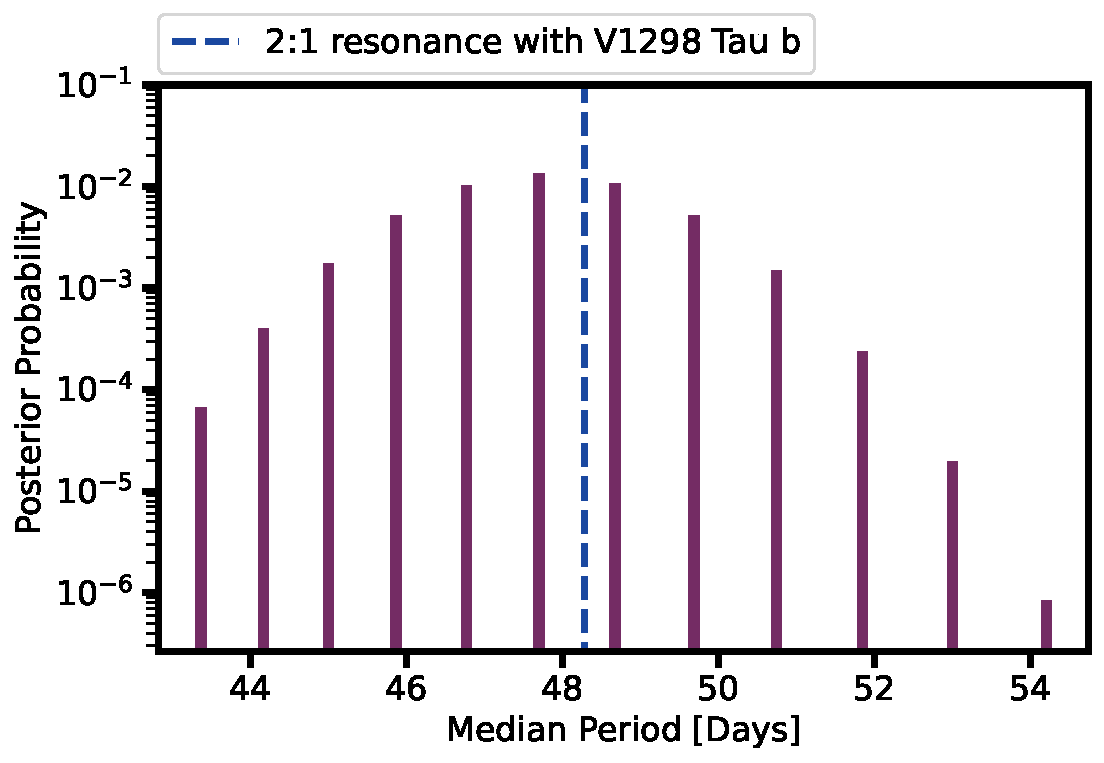
\includegraphics[width=0.45\textwidth,trim={0.25cm 0 0cm 0}]{static/periode.pdf}
\caption{Our calculated posterior probability to constrain the period of \planete using transit timings from \textit{K2} and \tess. We tested discrete periods from $38-60$\,days and find the most likely period to be 45.003~days. The 2:1 resonance (48.28~days) with \planetb is plotted as the dashed vertical line. \href{https://github.com/afeinstein20/v1298tau_tess/blob/main/notebooks/V1298Tau_e.py}{\github}} \label{fig:period_e}
\end{center}
\end{figure}
%%%%%%%%%%%%%%%%%%%%%%%%%%%%%%%%%%%%%%%%%%%%%%%%%%%%%%%

Independent ground-based monitoring of the system may be able to observe another transit of the outermost known planet in this system. Using the Transit Service Query Form on the NASA Exoplanet Archive \citep{Akeson2013}, we provide several potential transit midpoint events, given the top 5 most-likely periods for \planete, at the end of Table~\ref{tab:table}.

\section{Differences in Measured Radii} \label{sec:radii}

We compare the differences in transit $R_p/R_\star$ between the \textit{K2} and \tess\ data in Figure~\ref{fig:compare}. We masked regions in the light curve where transits overlapped. The residuals of the \tess\ light curve with our model (color) are plotted as well. For \planetknown, the transit radii are smaller in the \tess\ data, while only the measured radius for \planete is larger in the \tess\ data (Figure~\ref{fig:compare}, bottom panel).


\subsection{Radii of \planetknown}

%%%%%%%%%%%%%%%%%%%%%%%%%%%%%%%%%%%%%%%%%%%%%%%%%%%%%%%
\begin{figure*}[!htb]
\begin{center}
\includegraphics[width=\textwidth,trim={0.25cm 0 0 0}]{static/combined_together.pdf}
\caption{Left: Phase-folded \tess\ data (gray) with the new best-fit model (color) compared to the original \textit{K2} data (black). The residuals between the \tess\ data and each fit are shown underneath. Top right: A comparison of measured $R_p/R_\star$ are presented with a 1-to-1 line plotted in black for reference. The transit depths for \planetknown are shallower in the new \tess\ data, while the transit depth for \planete is deeper. Bottom right: The change in $R_p/R_\star$ as a function of pixel for \planetb (left) and \planete (right) overlaid with a sky image of \sname taken with the Digitized Sky Survey (DSS) r-band. We speculate the variation in transit depths could be due to contamination from nearby bright stars or starspot crossing events. \href{https://github.com/afeinstein20/v1298tau_tess/blob/main/src/figures/dilution_check.py}{\github}} \label{fig:compare}
\end{center}
\end{figure*}
%%%%%%%%%%%%%%%%%%%%%%%%%%%%%%%%%%%%%%%%%%%%%%%%%%%%%%%

A shallower transit depth at redder wavelengths is supported by the dusty outflow model presented in \citep{wang19}, while transits in the optical probe lower atmospheric pressures, resulting in larger transit depths \citep{gao20}. Therefore, the difference in transit depths could be due to the difference in bandpass wavelength coverage between \textit{Kepler} \citep[400-900~nm;][]{Howell2014} and \tess\ \citep[600-1000~nm;][]{Ricker2015}. 

The ability of a planet to retain hazes/transition hazes is negatively correlated with its equilibrium temperature, $T_{eq}$, internal temperature $T_{int}$, and positively correlated with mass, $M_{core}$. \allplanets have calculated $T_{eq} < 1000$\,K, assuming an albedo~=~0 \citep{David2019a}. Young planets are believed to have high $T_{int}$ due to ongoing gravitational contraction \citep{gu04}. The combination of these two parameters make these planets more likely to host extended high-altitude hazes in their atmospheres, while outflow winds lead to the formation of transition hazes \citep{gao20}. 

However, it is more likely we are seeing either contamination/dilution from another nearby star or the presence of starspots. As highlighted in Figure~\ref{fig:tpf}, there is a bright (\tess\ magnitude $<$ 14) just next to \sname. Since we did not include this source in our light curve PSF-modeling, it is possible there is some light from this source in our data, therefore making the transits of \planetknown appear $\sim 10$\% shallower in our \tess\ data than the original \textit{K2} measurements. The \tess\ Input Catalog \citep{stassun18} lists a contamination value of 0.315 for \sname, which could sufficiently produce the decrease in transit depths presented here. 

We check for signs of dilution by creating light curves for individual pixels around \sname and measure the transit depths of \planetb and \planete (Figure~\ref{fig:compare}). We localized a 1-day window around each transit and computed the a $\chi^2$ fit using a transit model computed with \texttt{batman} \citep{Kreidberg15} and an underlying 2\textsuperscript{nd} order polynomial. We find the transit depths to decrease falling off of the pixels centered on \sname. While fitting the \tess\ PSF with a 2D Gaussian function is a reasonable approximation, it is not the perfect model. It is possible that this light curve is diluted from nearby stars, including TIC~15756226, which is the closest (separation $= 49.15\arcsec$) star with $T_\textrm{mag} = 13.09$.

A change in transit depth could additionally be due to starspots, either from a nearby source or from the surface of \sname. In the context of starspots on \sname, both starspot/active region crossing events, where the planets directly transit over these inhomogeneities, or asymmetric starspots/active region distributions located off the transit chord could lead to differences in transit depths and shapes. In the case of starspot crossing events, we would expect to see added variability to the transit shape. Assuming we are not underestimating our error bars, this is readily seen in the transit of \planetb, both in the \tess\ and \textit{K2} data (Figure~\ref{fig:compare}). 


\subsection{Radius of \planete}

Contrary to \planetknown, we measure a transit radius that is $\sim 3\sigma$ larger in the new \tess\ data than what was found in the original \textit{K2} data \citep{David2019a}. The difference in radii could be consistent with a large scale height, low mean-molecular weight atmosphere around \planete \citep{deMooij12}. It is also possible the atmosphere of \planete is dominated by species with stronger absorption features at longer wavelengths, such as CO, H$_2$O, and CH$_4$ \citep{carter09}. 

We find it is more likely that the original single transit of \planete was filled-in via spot-crossing events, making it appear shallower in the \textit{K2} observations. Young stars are known to have very high spot coverage, anywhere from 30-80\% \citep[][]{grankin99, gully17, feinstein20}. It is therefore likely the surface of \sname is dominated by stellar inhomogeneities. This hypothesis is further strengthened by comparing the transit shape between the two data sets (Figure~\ref{fig:compare}). The center of the \textit{K2} transit is deeper than the edges and is consistent with the most recently observed transit depth. The lower contrast in starspot signals at longer wavelengths could potentially explain why the transit depth is consistent deeper in the \tess\ observations. Additionally, there is noise in-transit in the \tess\ data that could potentially be more starspot crossing events.


Future \tess\ 20-second and 2-minute data may have the temporal resolution needed to yield insight into if there is evidence of starspot crossing events. Our transit of \planete from the FFIs shows some structure. At the 10-minute cadence, it is hard to rule out noise as the source of this structure. However if there is such evidence of starspot crossings in the higher-cadence \tess\ observations, it would be interesting if any of the events dilutes the transit enough to result in a similar transit depth to that which was seen in \textit{K2}. 

\section{Conclusions} \label{sec:conclusions}

We present new ephemerides for all four known planets in the \sname system. We detected a second transit of \planete; this new transit time in combination from the transit observed with \textit{K2} allowed us to place tighter constraints on the period of the outermost planet. Our revised radius for planet e makes it now the largest planet in the system and extends an intriguing size--separation correlation in \sname such that planet size increases monotonically with separation.

We find the transit depths of \planetknown as observed by \tess\ are shallower than those observed by \textit{K2} by $1-2\sigma$, with the exception of \planete, which is $\sim 3\sigma$ larger. While this could possibly be due to ongoing dusty outflows that make the transit depth appear shallower, it is more likely the differences are due to starspot crossing events, asymmetric starspots off the transit chord, or contamination from nearby faint stars in the same \tess\ pixels are \sname. Modeling potential starspot crossing events could be accomplished using the 2-minute and 20-second cadence light curves, which will be available in the coming months.

The youth of these planets could additionally favor hosting haze-dominated atmospheres. However, without mass estimates for \allplanets, it is difficult to determine if this is the cause of the different transit depths measured between the \textit{K2} data and our presented work. Radial velocity mass measurements are challenging for young planets due to underlying stellar activity. A more promising approach to measuring the masses would be through TTVs \citep{agol18}. A full TTV analysis \textit{K2}, \textit{Spitzer}, and \tess\ transit photometry is presented in Livingston et al. (in prep). Additional transits at longer wavelengths or simultaneous multi-band photometry or spectroscopy could corroborate the potential of constraining the properties of these young atmospheres.

%The Python code used to access the data, process and model the light curve, and reproduce the tables and figures are made publicly available.\footnote{\url{https://github.com/afeinstein20/v1298tau_tess}}

\begin{acknowledgments}
We thank Rodrigo Luger for developing \texttt{showyourwork!} \citep{luger21} and helping us debug this letter, and we thank Chas Beichman and Sarah Blunt for helpful comments on our \tess\ proposal (DDT 036). ADF acknowledges support from the National Science Foundation Graduate Research Fellowship Program under Grant No. (DGE-1746045).

This research has made use of NASA's Astrophysics Data System Bibliographic Services. This research made use of Lightkurve, a Python package for \textit{Kepler} and \tess\ data analysis \citep{lightkurve}.

\end{acknowledgments}


\begin{deluxetable*}{l r r r r}[hbtp]
\tabletypesize{\footnotesize}
\tablecaption{\sname light curve fitting results and predicted ground-based transit midpoint events for \planete. \label{tab:table}}
\tablehead{\\
\hline\
\textit{Star} & \textit{Value} & \textit{Prior} &  & \\
\hline
$R_\star [R_\odot]$ & $1.33_{-0.03}^{+0.04}$ & $\mathcal{G}(1.305, 0.07)$ & & \\
$M_\star [M_\odot]$ & $1.095_{-0.047}^{+0.049}$ & $\mathcal{G}(1.10, 0.05)$& & \\
$u_1$ & $0.32_{-0.19}^{+0.20}$ & $\mathcal{U}[0, 1]$ in $q_1$ & & \\
$u_2$ & $0.16_{-0.29}^{+0.31}$ & $\mathcal{U}[0, 1]$ in $q_2$ & & \\
$P_{rot}$ [days] & $2.97_{-0.04}^{+0.03}$ & $\mathcal{G}($ln$ 2.87, 2)$ & & \\
ln($Q_0$) & $0.72_{-0.21}^{+0.24}$ & $\mathcal{H}(\sigma=2)$ & & \\
$\Delta Q_0$ & $4.09 \pm 1.01$ & $\mathcal{G}(0, 2)$ & & \\
f [ppt] & $0.85_{-0.19}^{+0.11}$ & $\mathcal{U}[0.1, 1]$ & & \\
\hline\
\textit{Light Curve} & \textit{Value} & \textit{Prior} &  & \\
\hline
$\mu$ & $-1.66_{-9.28}^{+9.42}$& $\mathcal{G}(0, 10)$ & &\\
ln($\sigma_l$) & $-2.499_{-4.463}^{+4.444}$ & $\mathcal{G}($ln$(0.1\sigma_\textrm{flux}), 10)$ & & \\
ln($\sigma_j$) & $-1.36_{-5.06}^{+4.96}$ & $\mathcal{G}($ln$(0.1\sigma_\textrm{flux}), 10)$ & & \\
\hline\
\textit{Planets} & \textit{c} & \textit{d} & \textit{b} & \textit{e}\\
\hline
$T_0$ [BKJD - 2454833] & $4648.1576_{-0.0034}^{+0.0042}$ & $4645.4113_{-0.0021}^{+0.0023}$ & $4648.0913_{-0.0013}^{+0.0015}$ & $4648.7975_{-0.0014}^{+0.0012}$ \\
P [days]               & $8.2479_{-0.0019}^{+0.0016}$ & $12.4030_{-0.0016}^{+0.0020}$ & $24.1382_{-0.0022}^{+0.0019}$ & $50.29 \pm 6.62$ \\
$R_p/R_\star$          &  $0.0339 \pm 0.0014$ & $0.0405 \pm 0.0016$ & $0.0635 \pm 0.0019$ & $0.0685 \pm 0.0026$ \\
$b$                    &  $0.14_{-0.10}^{+0.14}$ & $0.19_{-0.13}^{+0.12}$ & $0.45_{-0.04}^{+0.05}$ & $0.48_{-0.07}^{+0.06}$ \\
T$_{14}$ [hours]        &  $4.66_{-0.43}^{+0.49}$ & $5.59_{-0.53}^{+0.57}$ & $6.42_{-0.61}^{+0.66}$ & $7.44_{-0.71}^{+0.79}$  \\
$R_p [R_\oplus]$       & $4.92_{-0.24}^{+0.26}$ & $5.88_{-0.27}^{+0.29}$ & $9.21_{-0.36}^{+0.40}$ & $9.94_{-0.45}^{+0.49}$\\
$R_p [R_J]$       & $0.44 \pm 0.02$ & $0.52 \pm 0.02$ & $0.82 \pm 0.03$ & $0.89 \pm 0.04$\\
\hline\
\textit{Priors} & \textit{c} & \textit{d} & \textit{b} & \textit{e}\\
\hline
$T_0$ [BKJD - 2454833] & $\mathcal{G}(4648.53,0.1)$ & $\mathcal{G}(4645.4,0.1)$ & $\mathcal{G}(4648.1,0.1)$ & $\mathcal{G}(4648.8,0.1)$ \\
log($P$ [days]) & $\mathcal{G}($ln$ 8.25, 1)$ & $\mathcal{G}($ln$ 12.40, 1)$& $\mathcal{G}($ln$ 24.14, 1)$ & $\mathcal{G}($ln$ 36.70, 1)$\\
log(depth [ppt]) & $\mathcal{G}($ln$ 1.45, 0.1)$ & $\mathcal{G}($ln$ 1.90, 0.1)$ & $\mathcal{G}($ln$ 4.90, 0.1)$ & $\mathcal{G}($ln$ 3.73, 0.1)$ \\
$b$ & $\mathcal{U}[0, 1]$ & $\mathcal{U}[0, 1]$ & $\mathcal{U}[0, 1]$ & $\mathcal{U}[0, 1]$ \\
T$_{14}$ [days] & $\mathcal{G}($ln$ 0.19, 1)$ & $\mathcal{G}($ln$ 0.23, 1)$ & $\mathcal{G}($ln$ 0.27, 1)$ &  $\mathcal{G}($ln$ 0.31, 1)$\\
\hline \hline\
\\
\hline\
\planete \textit{P} [days] & Posterior Prob. & Mountain Standard Time [UTC-7] & Pacific Time [UTC-8] & Hawaiian Time [UTC-10] \\
\hline
45.003 & $0.0488$ & 23-12-2021 00:17 & 22-12-2021 23:17 & 22-12-2021 21:17 \\
    &  & 06-02-2022 00:25 & 05-02-2022 23:25 & 05-02-2022 21:25 \\
    &  & 23-03-2022 01:30 & 23-03-2022 00:30 & 22-03-2022 21:30\\
    \hline\
45.869 & $0.0488$ & 24-12-2021 17:55 & --- & ---\\
\hline\
44.170 & $0.0487$ & --- & --- & 21-12-2021 05:42\\
    &  & 19-03-2022 17:31 & --- & --- \\
\hline\
40.427 & $0.0485$ & 13-12-2021 20:42 & 13-12-2021 19:42 & 13-12-2021 17:42 \\
    &  & ---  & --- & 23-01-2022 05:57 \\
    &  & 04-03-2022 17:12 & --- & --- \\
\hline\
43.367 & $0.0484$ & 20-12-2021 17:49 & --- & ---\\
    &  & 01-02-2022 02:38 & 01-02-2022 01:38 & 31-01-2022 23:38 \\
    & & --- & --- & 16-03-2022 08:26
}
\startdata
\enddata
\tablecomments{Priors are noted for parameters that were directly sampled. The distributions are as follows -- $\mathcal{G}$: Gaussian; $\mathcal{H}$: Half-normal; $\mathcal{U}$: Uniform. $\sigma_\textrm{flux}$ is the standard deviation of the light curve.}
\tablecomments{Transit dates were calculated using the Transit Service Query Form on the NASA Exoplanet Archive \citep{Akeson2013}. These transit times take into account Daylight Savings time zone changes within the United States.}
\end{deluxetable*}


%\vspace{5mm}
\facilities{\tess\ \citep{Ricker2015}, \textit{Kepler} \citep{Howell2014}}


\software{\texttt{exoplanet} \citep{exoplanet2021},
          \texttt{EVEREST 2.0} \citep{luger18},
          \texttt{lightkurve} \citep{lightkurve},
          \texttt{matplotlib} \citep{matplotlib},
          \texttt{PyMC3} \citep{Salvatier16},
          \texttt{starry} \citep{luger19},
          \texttt{theano} \citep{theano},
          \texttt{tica} \citep{fausnaugh20},
          \texttt{showyourwork!} \citep{luger21},
          \texttt{astropy} \citep{astropy:2013, astropy18},
          \texttt{astroquery}\citep{astroquery19},
          \texttt{numpy} \citep{numpy},
          \texttt{celerite2} \citep{dfm17},
          \texttt{batman} \citep{Kreidberg15}
          }



\bibliography{main}
\bibliographystyle{aasjournal}

\end{document}
